\documentclass[xcolor={dvipsnames,rgb}]{beamer}

\beamertemplatenavigationsymbolsempty

\usepackage{tikz}
\usepackage{amsmath}
\usepackage{amssymb}
\usepackage{mathtools}

\usetikzlibrary{positioning}
\usetikzlibrary{backgrounds}
\usetikzlibrary{tikzmark}
\usetikzlibrary{shapes,arrows,calc}

\newcommand{\highlight}[2]{\colorbox{#1}{$\mathstrut #2$}}

\definecolor{variable}{HTML}{999999}
\definecolor{operator}{HTML}{bbbbbb}
\definecolor{vtrue}{HTML}{66ff66}
\definecolor{vfalse}{HTML}{ff6666}
\definecolor{rtrue}{HTML}{aaffaa}
\definecolor{rfalse}{HTML}{ffaaaa}

\tikzstyle{into} = [draw, -triangle 45, shorten >=0pt]

\tikzstyle{label} = [minimum height=2em, minimum width=2em]
\tikzstyle{var} = [draw, rectangle, minimum height=2em, minimum width=2em, fill=variable]
\tikzstyle{oper} = [draw, rectangle, minimum height=2em, minimum width=2em, fill=operator]
\tikzstyle{it} = [draw, diamond, minimum height=2em, minimum width=2em, fill=vtrue]
\tikzstyle{if} = [draw, circle, minimum height=2em, minimum width=2em, fill=vfalse]
\tikzstyle{ot} = [draw, diamond, minimum height=2em, minimum width=2em, fill=rtrue]
\tikzstyle{of} = [draw, circle, minimum height=2em, minimum width=2em, fill=rfalse]



% https://i.stack.imgur.com/2X1Jv.png
\colorlet{ca}{Peach!30}
\colorlet{co}{Goldenrod!30}
\colorlet{cn}{Tan}
\colorlet{ci}{Sepia!30}


\begin{document}

\begin{frame}{Evaluation of a \textit{Boolean expression}}

  % https://github.com/st--/annotate-equations/blob/main/examples/demo_manual_annotate_beamer.tex#L55

  
  \onslide<+->{
    \begin{equation*}
      \text{Expression:} \,
      \tikzmarknode{notand}{\highlight{cn}{\neg}}
      \tikzmarknode{aandb}{\highlight{ca}{(a \wedge b)}}
      \tikzmarknode{final}{\highlight{ci}{\rightarrow}}
      \tikzmarknode{cord}{\highlight{co}{(c \vee d)}}
    \end{equation*}
  }
  
  \begin{center}
    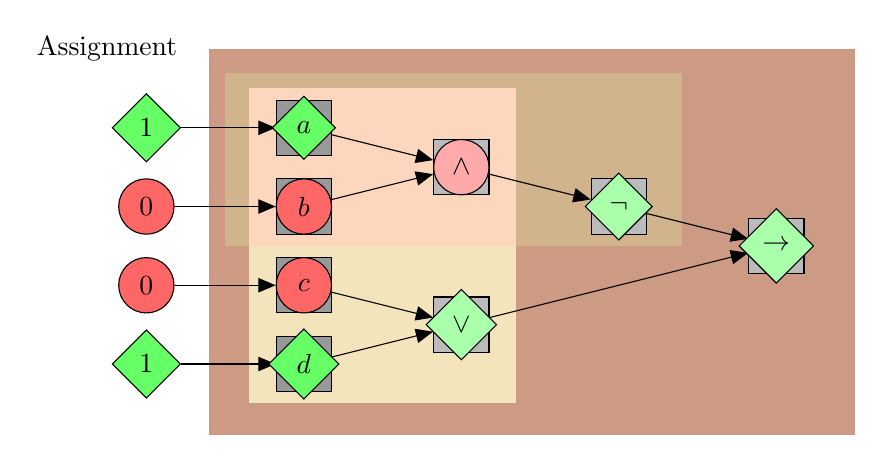
\begin{tikzpicture}
      
      \onslide<17-18,32-35>{\fill [fill=ci] (-1.2, 0.1) rectangle (7, 5);}     
      \onslide<13-15,30-35>{\fill [fill=cn] (-1, 2.5) rectangle (4.8, 4.7);}      
      \onslide<7-8,24-35>{\fill [fill=ca] (-0.7, 2.5) rectangle (2.7, 4.5);}
      \onslide<10-11,30-35>{\fill [fill=co] (-0.7, 0.5) rectangle (2.7, 2.5);}      
      
      % variables
      \onslide<2->{\node[var](a) at (0, 4){$a$};}
      \onslide<3->{\node[var](b) at (0, 3){$b$};}
      \onslide<4->{\node[var](c) at (0, 2){$c$};}
      \onslide<5->{\node[var](d) at (0, 1){$d$};}
      
      % operators
      \onslide<6->{\node[oper](and) at (2, 3.5) {$\wedge$};}
      \onslide<9->{\node[oper](or) at (2, 1.5) {$\vee$};}
      \onslide<12->{\node[oper](not) at (4, 3) {$\neg$};}
      \onslide<16->{\node[oper](impl) at (6, 2.5) {$\rightarrow$};}

      % equation arrows
      \onslide<6->{\draw [into] (a) -- (and);}
      \onslide<6->{\draw [into] (b) -- (and);}   
      \onslide<9->{\draw [into] (c) -- (or);}
      \onslide<9->{\draw [into] (d) -- (or);}
      \onslide<12->{\draw [into] (and) -- (not);}
      \onslide<16->{\draw [into] (or) -- (impl);}
      \onslide<16->{\draw [into] (not) -- (impl);}           

      % value assignment
      \onslide<19->{\node at (-2.5, 5) {Assignment};}

      % first part
      \onslide<20->{\node[it](av) at (-2, 4){1};}
      \onslide<22->{\node[if](bv) at (-2, 3){0};}

      % step 1
      \onslide<21->{\draw [into] (av) -- (a);}
      \onslide<23->{\draw [into] (bv) -- (b);}      
      \onslide<24->{\node[of](and2) at (2, 3.5) {$\wedge$};}
      \onslide<21->{\node[it](a2) at (0, 4){$a$};}
      \onslide<23->{\node[if](b2) at (0, 3){$b$};}

      % second part
      \onslide<25->{\node[if](cv) at (-2, 2){0};}
      \onslide<27->{\node[it](dv) at (-2, 1){1};}

      % step 2
      \onslide<26->{\draw [into] (cv) -- (c);}
      \onslide<28->{\draw [into] (dv) -- (d);}
      \onslide<29->{\node[ot](or2) at (2, 1.5) {$\vee$};}
      \onslide<26->{\node[if](c2) at (0, 2){$c$};}
      \onslide<28->{\node[it](d2) at (0, 1){$d$};}
      
      % step 3
      \onslide<30->{\node[ot](not2) at (4, 3) {$\neg$};}

      % step 4
      \onslide<32->{\node[ot](impl2) at (6, 2.5) {$\rightarrow$};}
      
    \end{tikzpicture}

    \onslide<34-38>{Under the given \textit{assignment} to the variables, this expression evaluates to \textbf{true}.}
    
  \end{center}
\end{frame}


\end{document}
